% Straight up stealing preamble from Eli Holmes 
%%%%%%%%%%%%%%%%%%%%%%%%%%%%%%%%%%%%%%START PREAMBLE THAT IS THE SAME FOR ALL EXAMPLES
\documentclass{article}

%Required: You must have these
\usepackage{Sweave}
\usepackage{graphicx}
\usepackage{tabularx}
\usepackage{hyperref}

%Strongly recommended
  %put your figures in one place
 
%you'll want these for pretty captioning
\usepackage[small]{caption}
\setkeys{Gin}{width=0.8\textwidth}  %make the figs 50 perc textwidth
\setlength{\captionmargin}{30pt}
\setlength{\abovecaptionskip}{0pt}
\setlength{\belowcaptionskip}{10pt}
% manual for caption  http://www.dd.chalmers.se/latex/Docs/PDF/caption.pdf

%Optional: I like to muck with my margins and spacing in ways that LaTeX frowns on
%Here's how to do that
 \topmargin -1.5cm        
 \oddsidemargin -0.04cm   
 \evensidemargin -0.04cm  % same as oddsidemargin but for left-hand pages
 \textwidth 16.59cm
 \textheight 21.94cm 
 %\pagestyle{empty}       % Uncomment if don't want page numbers
 \parskip 7.2pt           % sets spacing between paragraphs
 %\renewcommand{\baselinestretch}{1.5} 	% Uncomment for 1.5 spacing between lines
\parindent 0pt		  % sets leading space for paragraphs
\usepackage{setspace}
%\doublespacing

%Optional: I like fancy headers
\usepackage{fancyhdr}
\pagestyle{fancy}
\fancyhead[LO]{Question: How does active warming affect microclimate?}
\fancyhead[RO]{2016}
 
%%%%%%%%%%%%%%%%%%%%%%%%%%%%%%%%%%%%%%END PREAMBLE THAT IS THE SAME FOR ALL EXAMPLES

%Start of the document
\begin{document}

% \SweaveOpts{concordance=TRUE}

\title{Question: How does active warming affect microclimate?} % Reconciling Experimental and Observational Approaches for Climate Change Impacts
\author{A. K. Ettinger}
%\date{\today}
\maketitle  %put the fancy title on
%\tableofcontents      %add a table of contents
%\clearpage
%%%%%%%%%%%%%%%%%%%%%%%%%%%%%%%%%%%%%%%%%%%%%%%%%%%
Here are a series of basic graphs and analyses, with my initial interpretation, of how experimental active warming affects climate. We start by comparing sham (temptreat="0" in "expclim.csv") and  ambient plots (temptreat="ambient" in "expclim.csv") to get a sense of how simply having the warming structures in place affects microclimate. 
First, some simple plots and models of how air temperature and soil temperature differs across these treatments at different sites:


\section {Air temperature}
Air temperature is HIGHER in the shams, compared with the ambient air. Below, mean daily air temperature is shown, for all sites for which these data are available (5). The pattern was consistent for minumum and maximum daily air temperature as well (also shown). Estimates with standard errors from linear mixed effect model with site as a random effect: ambient: 12.34 (SE:1.65); sham: 12.71 (SE: 1.64).

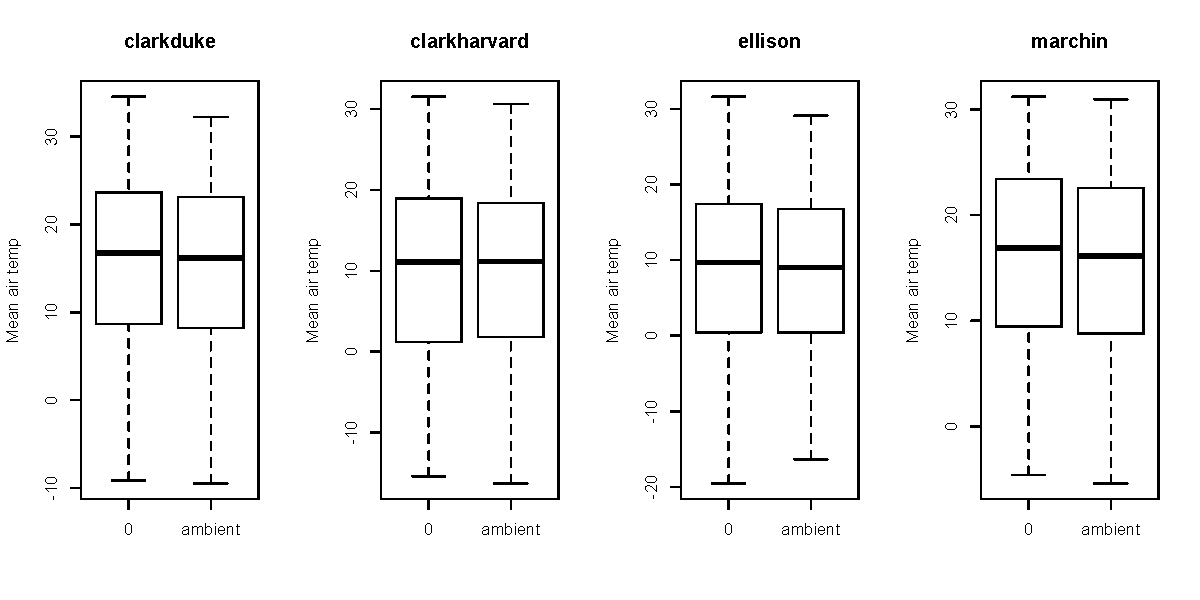
\includegraphics{Analyses/output/shamvambient_airtemp.pdf}
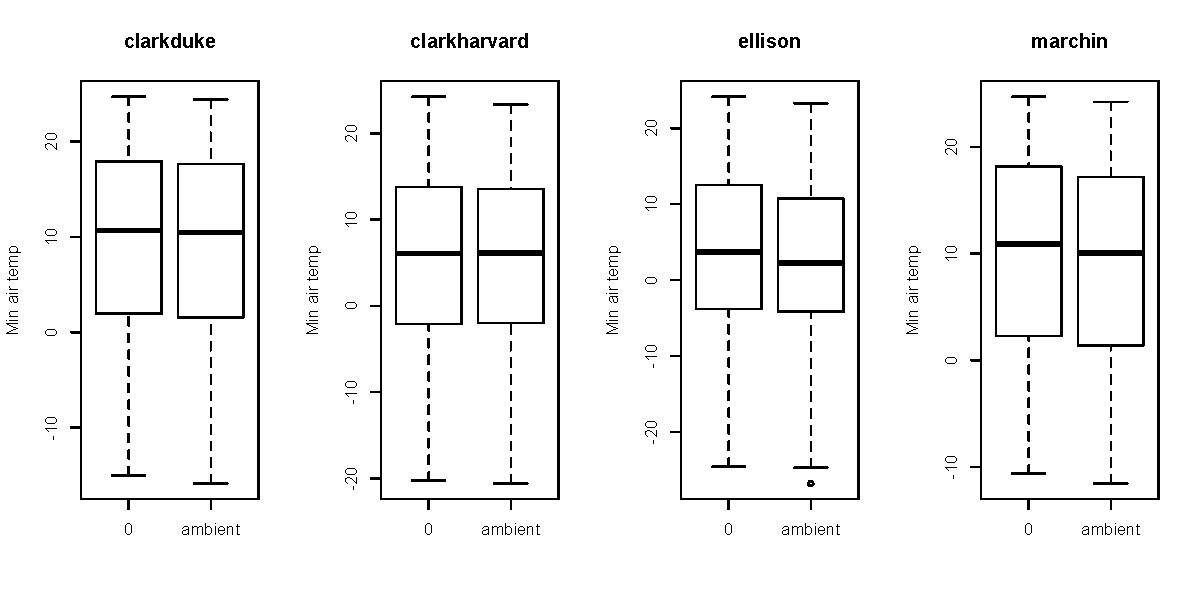
\includegraphics{Analyses/output/shamvambient_airtempmin.pdf}
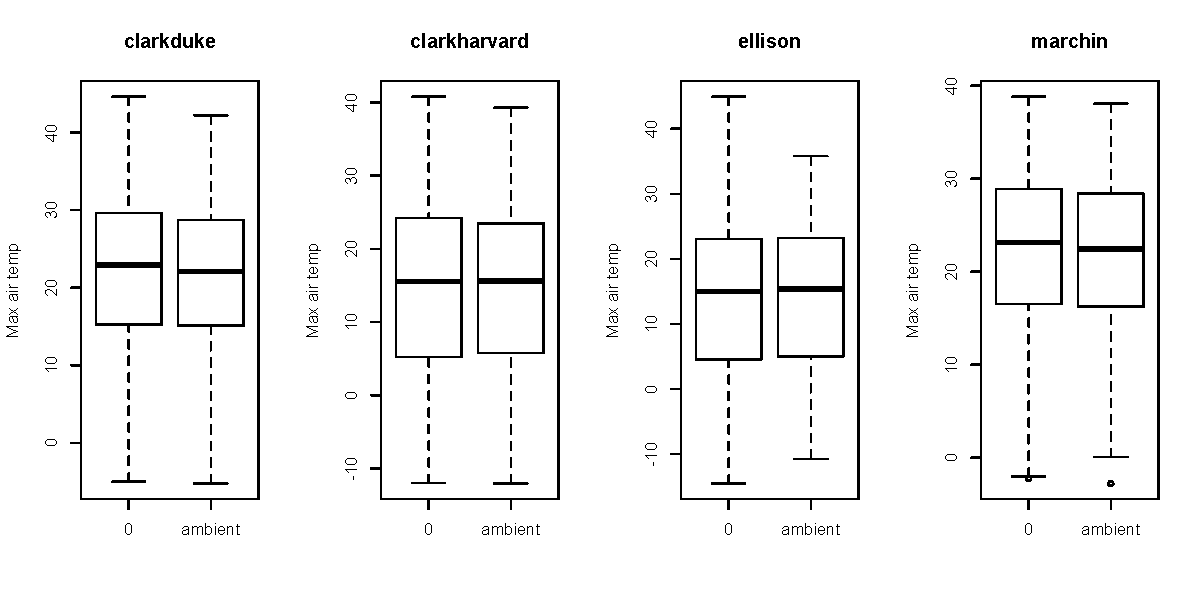
\includegraphics{Analyses/output/shamvambient_airtempmax.pdf}

\section {Soil temperature}
Soil temperature is LOWER in the shams, compared with the ambient air. Below, mean daily soil temperature (for the shallowest depth) is shown, for all sites for which these data are available, but the pattern was consistent for minumum and maximum daily soil temperatures as well. Estimates with standard errors from linear mixed effect model with site as a random effect: ambient: 11.73 (SE:1.36); sham: 11.31 (SE:1.37).

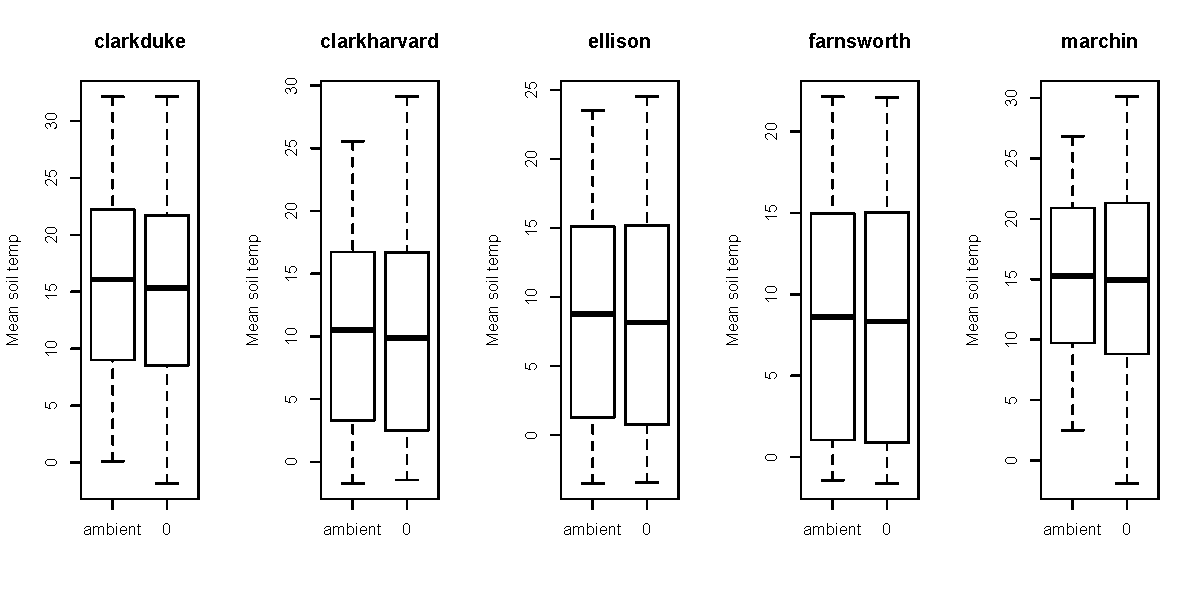
\includegraphics{Analyses/output/shamvambient_soiltemp.pdf}

\end{document}
